
%\hypertarget{aula-3}{%
%\chapter{Aula: 3}\label{aula-3}}



\hypertarget{processos}{%
\chapter{Processos}\label{processos}}

Ao visualizar um ícone de um programa na área de trabalho de um Sistema
Operacional (SO), o usuário está olhando para uma referência a uma
entidade passiva executável localizada na memória secundária. Ao clicar
duas vezes em cima do ícone, o programa \texttt{Loader} é acionado,
carregando o programa clicado para a memória principal, tornando-o uma
entidade ativa chamada de processo, o qual está inserido dentro de um
contexto de execução único em user mode, isolado dos demais processos.
Assim, um único programa é capaz de gerar múltiplos processos, como o
navegador de internet e as diversas abas abertas. De forma geral, um
processo divide a memória em quatro seções:

\begin{enumerate}
\def\labelenumi{\arabic{enumi}.}

\item
  Text: código executável.
\item
  Data: variáveis globais.
\item
  Heap: memória alocada dinamicamente em tempo de execução.
\item
  Stack: armazenamento temporário para, por exemplo, variáveis locais.
\end{enumerate}

Como é mostrado na Figura \ref{fig:Alocação de memória de um programa em C}, em um programa na linguagem C, as variáveis globais são separadas dentro da
seção \texttt{data} por utilizadas e não utilizadas. As variáveis dentro
da função \texttt{main} são alocadas na \texttt{stack}, sendo removidas,
automaticamente, após o uso. A seção \texttt{heap} é acessado pela
função \texttt{malloc(3)} (\emph{Memory Allocation}, ou alocação de
memória), o qual não remove os dados armazenados após o uso, devendo o
programador ter o cuidado de liberar a memória ocupada com a função
\texttt{free(3)}. Por fim, o código executável referente a esse programa
está armazenado na seção \texttt{text}. No programa em C, os argumentos
da função main são armazenados em uma seção específica.


\begin{figure}[h!]
\centering
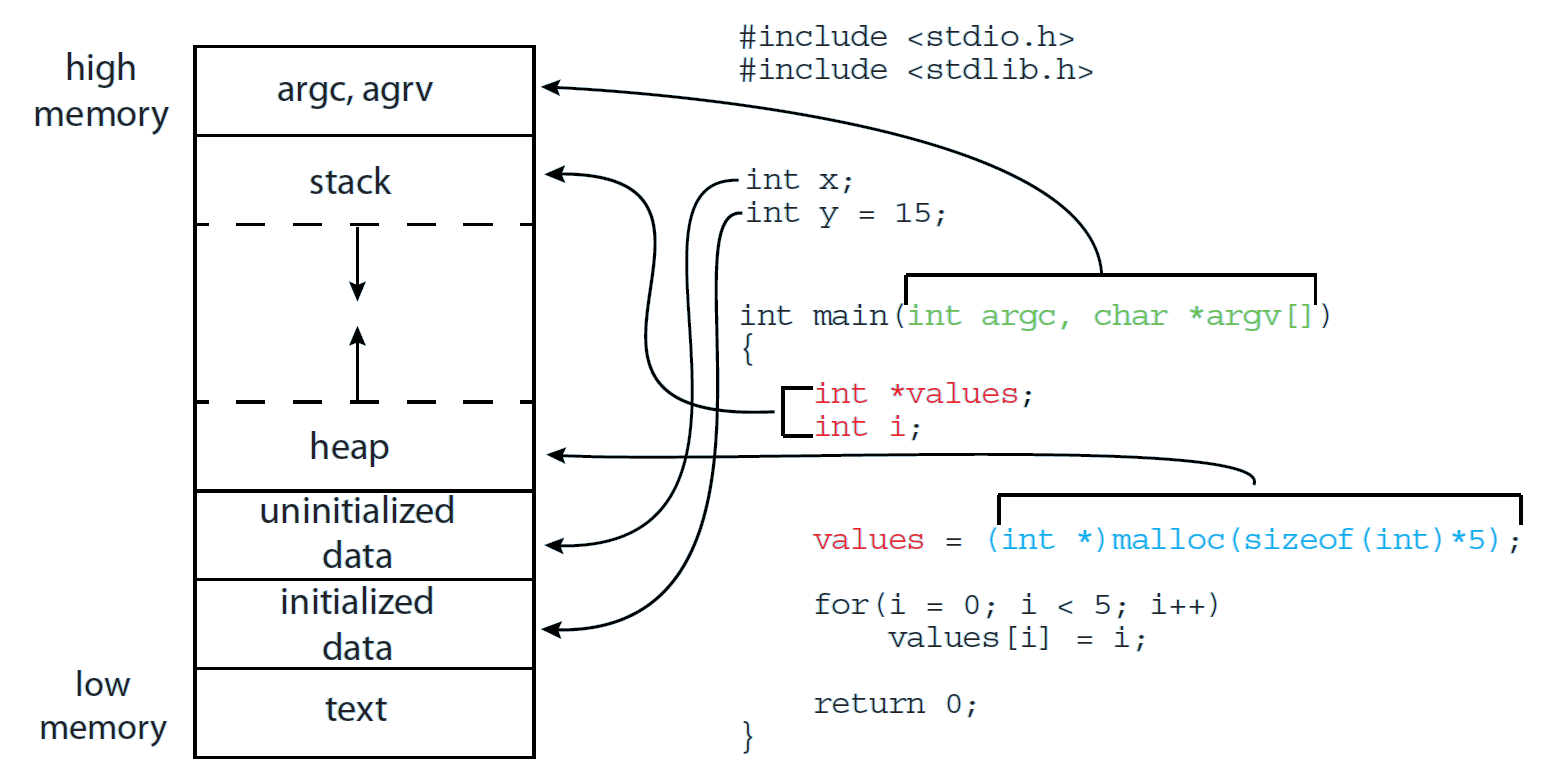
\includegraphics[keepaspectratio, width=12cm, height=9cm]{imagens/03/03 - Alocação de memória de um programa c.png}
\caption{Alocação de memória de um programa em C \\
Imagem retirada de: Silberschatz, A. Operating System Concepts, 10th,
página 108. \\}
\label{fig:Alocação de memória de um programa em C}
\end{figure}




Como a seção \texttt{text} e a \texttt{heap} crescem e diminuem
dinamicamente durante a execução do programa, existe um espaço, à ser
utilizado, entre ambos, de forma que a seção \texttt{stack}, sai de um
endereço superior da memória para um inferior, e o \texttt{heap} da
inferior para a superior. Na Figura \label{fig:Alocação de memória de um programa em C}, o endereço superior está chamado
de \emph{high-memory}, e o inferior de \emph{low-memory}. É papel do
sistema operacional de assegurar que ambas as seções não se sobreponham.

Cada processo é representado, no sistema operacional, pelo PCB
(\emph{Process Control Block}), uma lista encadeada contendo informações
como:

\begin{enumerate}
\def\labelenumi{\arabic{enumi}.}

\item
  \emph{Process state} - Podendo ser: \texttt{New}, \texttt{Running},
  \texttt{Waiting}, \texttt{Ready}, \texttt{Terminated}.
\item
  \emph{Program Counter} - Contador que indica o endereço da próxima
  instrução.
\item
  \emph{CPU registers} - Valor dos registradores da CPU.
\item
  \emph{CPU-scheduling information} - Informação sobre a prioridade do
  processo.
\item
  \emph{Memory-management information} - Informações sobre o
  gerenciamento de memória.
\item
  \emph{Accounting information} - Aqui está incluído dados como a
  quantidade de CPU usada.
\item
  \emph{I/O status information} - Informação sobre arquivos abertos,
  dispositivos I/O utilizados etc.
\end{enumerate}

\hypertarget{contexto-de-execuuxe7uxe3o}{%
\section{Contexto de Execução}\label{contexto-de-execuuxe7uxe3o}}

No código a seguir, temos a duas declarações da variável \texttt{a}.
Isso é possível pois cada declaração está dentro de um contexto de
execução diferente, de forma que cada função representa uma posição de
memória distinto, e, assim, seus conteúdos ocupam um espaço, ou
\texttt{Stack\ Frame}, específico da seção \texttt{stack}. Então, quando
uma função é chamada, o \texttt{Program\ Counter} é desviado para essa a
posição da memória, passando a executar as instruções lá inseridas, até
ser redirecionado de volta ao endereço inicial (no qual a função foi
chamada), descartando esse \texttt{Stack\ Frame}. O conteúdo contido no
\texttt{Stack\ Frame} descartado, não é removido da memória, por causa
do custo computacional de fazê-lo, fato gerador do chamado lixo de
memória (\texttt{Stack\ Frame} sem contexto), diminuindo, assim, o
\texttt{stack}. Quando um novo \texttt{Stack\ Frame} é concebido, esse
sobrescreve o lixo de memória anteriormente criado, aumentando o
\texttt{stack}.


\begin{minted}[mathescape, linenos]{c}

    void f()
    {
        int a = 4;
        printf("%d\n", a);
    }
    
    int main(int argc, char *argv[])
    {
        int a = 1;
        f();
        printf("%d\n", a);
    
    }

\end{minted}




Cada tipo de variável ocupa uma quantidade de bits específico, como
descriminado abaixo:

\begin{enumerate}
\def\labelenumi{\arabic{enumi}.}
\tightlist
\item
  \texttt{char:\ 8\ bits}
\item
  \texttt{int:\ 16\ bits}
\item
  \texttt{long:\ 32\ bits}
\item
  \texttt{float:\ 32\ bits}
\item
  \texttt{double:\ 64\ bits}
\end{enumerate}

\hypertarget{ponteiros}{%
\section{Ponteiros}\label{ponteiros}}

No programa mostrado na Figura \label{fig:Alocação de memória de um programa em C}, foi inicializada uma variável do typo
\texttt{int\ *}, o qual representa um ponteiro \texttt{int}. Os
ponteiros são baseados na ideia da indireção, ou seja, na referencia
indireta à outra posição da memória de tamanho \texttt{int} (16 bits).
Por ser uma referência, ele não ocupa o espaço referido, e sim um
específico para o seu tipo. No caso de uma arquitetura de 64 bits, o
ponteiro ocupa 8 bytes (64 bits).

O trecho de código da Figura \label{fig:Alocação de memória de um programa em C},


\begin{minted}[mathescape, linenos]{c}

    int *values;
    values = (int *) malloc(sizeof(int)*5);
    
    for(i = 0; i < 5; i++){
        values[i] = i; 
        // *(p + i) = i - Equivalente à: &values + i * sizeof(int) 
        // <= i
    }

\end{minted}


mostra que, o valor no qual está sendo referenciado pelo ponteiro
values, está no \texttt{heap} (jogado lá pela função \texttt{malloc(3)})
ocupando um espaço de 5 \texttt{int} (ou seja, 5 de 16 bits ou 80 bits).
Cada espaço desse é utilizado pela variável \texttt{i}, do tipo
\texttt{int}, fazendo, assim, com que o espaço referenciado por
\texttt{values} possa receber 5 do tipo \texttt{int}, como é utilizado
dentro do loop \texttt{for}, com a artimética de ocupação
\texttt{(\&values\ +\ i*sizeof(int))}, adicionado no código em forma de
cometário.

Podemos pensar na variável do ponteiro como um baú, no qual ao por
\texttt{*}, estamos acessando o conteúdo do baú, \texttt{\&} para o
endereço de memória que contém o valor referenciado,

No código a seguir, podemos ver 3 operações distintas com o ponteiro
\texttt{p}, as quais \texttt{\&} revela o endereço de memória do valor
``apontado'', \texttt{*} acessa o conteúdo da memória e, por fim,
\texttt{p} sem nenhum operador retorna o endereço da variável \texttt{p}
na \texttt{stack}.


\begin{minted}[mathescape, linenos]{c}

    int *values;
    int *p = malloc(sizeof(int)*4);
    
    p[0] = 10;
    printf("&p = %p/n", &p); // Endereço da referência (heap)
    printf("&p = %d/n", *p); // Conteúdo da referência
    printf("p = %p/n", p); // Endereço de p (Stack)

\end{minted}

